\newthought{\textbf{Cut Opy Mandalisa - 2020903430012 - TRKJ 3B}}

\newday{\textbf{1-2 Desember 2022- Instalasi dan Konfigurasi Hadoop}}
\begin{enumerate}
\item Kendala dan Solusi\\
% jelaskan kendala dan penyebab yang dialami saat mengikuti praktikum serta solusi atau langkah-langkah yang telah dilakukan
Pada Praktikum pertama yaitu penginstalan apache hadoop.kendala yang didapat tidak bisa membuka firefox kemudian solusinya dengan menginstal firefox baru.

\begin{figure}[!ht]
\includegraphics[width=\textwidth]{CutOpyMandalisa/01}
\caption{hasil dari cek hadoop service}
\label{gam:perkuliahan-25-11}
\end{figure}

\begin{figure}[!ht]
\includegraphics[width=\textwidth]{CutOpyMandalisa/02}
\caption{hasil cek hadoop service}
\label{gam:perkuliahan-25-11}
\end{figure}

\item Kesimpulan\\
% berikan kesimpulan dari praktikum yang telah dikerjkan
Behasil mendownload dan menginstal Apache hadoop dan sudah bisa dijalankan
\end{enumerate}


\newday{\textbf{08 Desember 2022-WordCount bawaan Hadoop}}
\begin{enumerate}

\item Kendala dan Solusi
\newpage
% jelaskan kendala dan penyebab yang dialami saat mengikuti praktikum serta solusi atau langkah-langkah yang telah dilakukan
Pada praktikum ini membuat program WordCount bawaan Hadoop. Pada melakukan praktikum tidak ada kendala hanya erorr dikarenakan salah memasukkan perintah.

\begin{figure}[!ht]
\includegraphics[width=\textwidth]{CutOpyMandalisa/03}
\caption{hasil WordCount bawaan Hadoop}
\label{gam:perkuliahan-25-11}
\end{figure}

\item Kesimpulan\\
% berikan kesimpulan dari praktikum yang telah dikerjkan
Pada praktikum ini untuk memahami proses cara kerja pada hadoop dalam memproses data input sehingga menghasilkan output.Wordcount merupakan program untuk menghitung jumlah kata dalam input.
\end{enumerate}


\newday{\textbf{09 Desember 2022-WordCount dengan Java}}
\begin{enumerate}
\item Kendala dan Solusi\\
% jelaskan kendala dan penyebab yang dialami saat mengikuti praktikum serta solusi atau langkah-langkah yang telah dilakukan
Pada praktikum ini membuat program WordCount dengan java.Pada saat melakukan praktikum terdapat error akan tetapi erorrnya disebabkan salah memasukkan perintah codingannya.solusinya harus lebih teliti saat memasukkan codingan tersebut.

\begin{figure}[!ht]
\includegraphics[width=\textwidth]{CutOpyMandalisa/04}
\caption{hasil wordCount dengan java}
\label{gam:perkuliahan-25-11}
\end{figure}

\item Kesimpulan\\
% berikan kesimpulan dari praktikum yang telah dikerjkan
Berhasil menjalankan program WordCount dengan java.
\end{enumerate}


\newday{\textbf{15 Desember 2022- Instalasi Apache Spark}}
\begin{enumerate}
\item Kendala dan Solusi\\
% jelaskan kendala dan penyebab yang dialami saat mengikuti praktikum serta solusi atau langkah-langkah yang telah dilakukan
pada praktikum ini yaitu penginstalan apache spark. Kendalanya terdapat pada verifikasi hasil installasi spark yang dimana pada saat mengetik perintahnya lupa menambahkan -- dan sekarang sudah berhasil penginstalannya.

\begin{figure}[!ht]
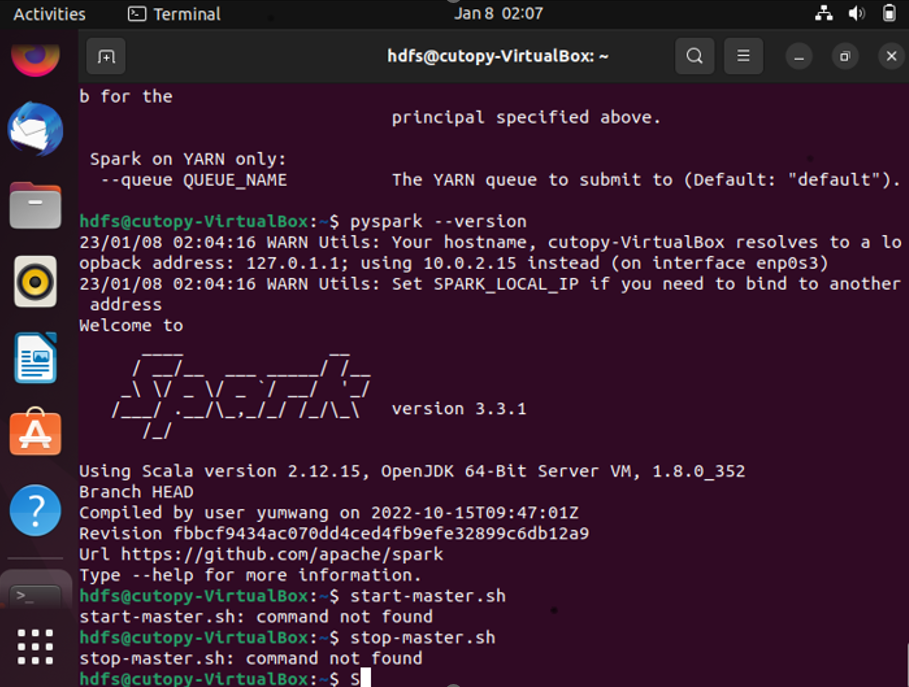
\includegraphics[width=\textwidth]{CutOpyMandalisa/05}
\caption{hasil Penginstalasi Apache Spark (PySpark)}
\label{gam:perkuliahan-15-12}
\end{figure}

\item Kesimpulan\\
% berikan kesimpulan dari praktikum yang telah dikerjkan
Berhasil menginstall Apache Spark yang sudah bisa dijalankan
\end{enumerate}


\newday{\textbf{16 Desember 2022- WordCount Python}}
\begin{enumerate}
\item Kendala dan Solusi\\
% jelaskan kendala dan penyebab yang dialami saat mengikuti praktikum serta solusi atau langkah-langkah yang telah dilakukan
Pada Praktikum ini kendalanya di mencoba program di local dan pada saat menjalankan program menggunakan hadoop dan sekarang sudah mendapatkan solusinya

\begin{figure}[!ht]
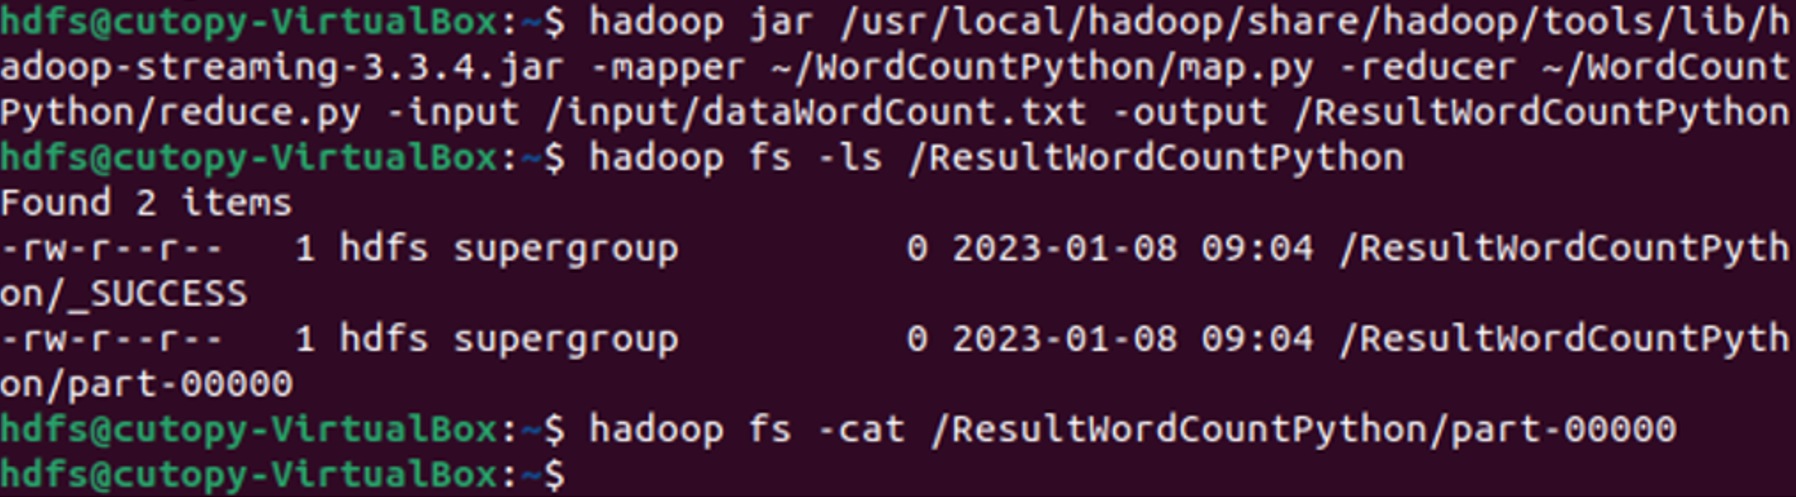
\includegraphics[width=\textwidth]{CutOpyMandalisa/06}
\caption{hasil WordCount Python}
\label{gam:perkuliahan-16-12}
\end{figure}

\item Kesimpulan\\
% berikan kesimpulan dari praktikum yang telah dikerjkan
Berhasil menjalankan programnya meski ada kendala saat mengetik perintahnya tetapi ketika memperhatikan lagi dengan benar perintah sudah benar maka ketika di dijalankan perintah tersebut sudah bisa.
\end{enumerate}

\newday{\textbf{22 Desember 2022- WordCount PySpark}}
\begin{enumerate}
\item Kendala dan Solusi\\
% jelaskan kendala dan penyebab yang dialami saat mengikuti praktikum serta solusi atau langkah-langkah yang telah dilakukan
Pada saat melakukan praktikut ini terdapat pada saat menjalankan program menggunakan pyspark,ternyata salahnya di salah pengetikan yang tidak teliti,sekarang sudah menemukan solusi dan programnya sudah berhasil

\begin{figure}[!ht]
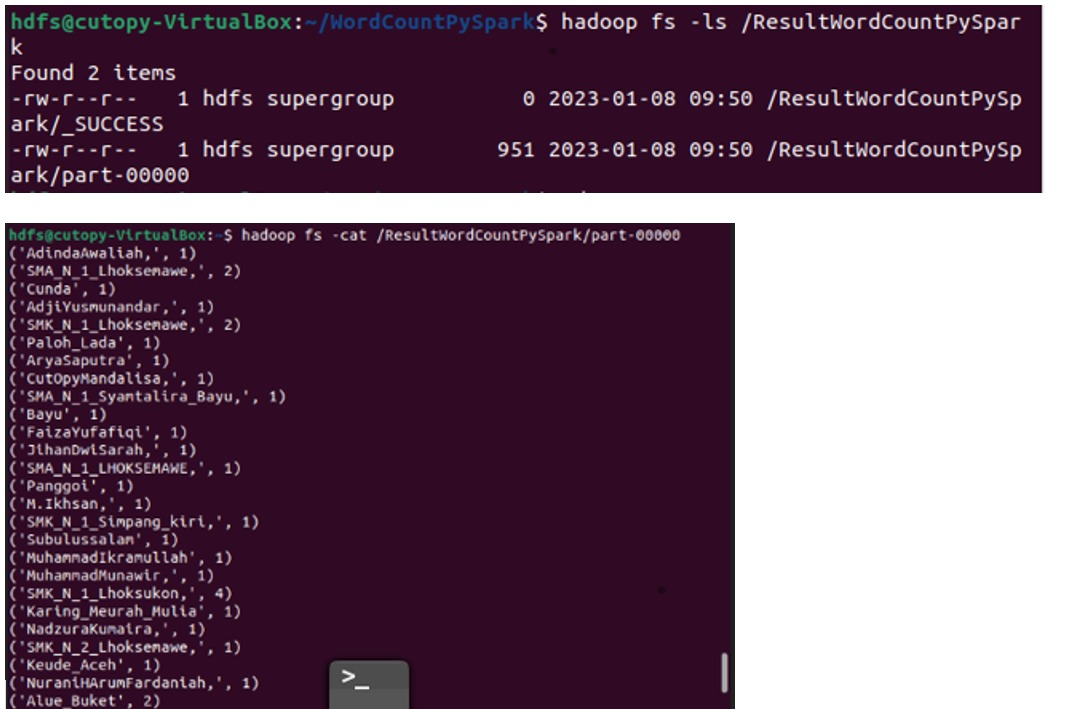
\includegraphics[width=\textwidth]{CutOpyMandalisa/07}
\caption{hasil WordCount PySpark }
\label{gam:perkuliahan-22-12}
\end{figure}

\item Kesimpulan\\
% berikan kesimpulan dari praktikum yang telah dikerjkan
Berhasil melakukan Program WordCount dengan PySpark
\end{enumerate}

\newday{\textbf{05 Januari 2023-Tugas individu program machine learning dengan pyspark }}
\begin{enumerate}
\item Kendala dan Solusi\\
% jelaskan kendala dan penyebab yang dialami saat mengikuti praktikum serta solusi atau langkah-langkah yang telah dilakukan
kendalanya pada penginstalan package dan pada saat menentukan nilai k dengan metode silhoutte,grafik tidak muncul,seharusnya setelah perintah plt.show() akan muncul grafik,belum ditemukan solusinya. pada saat menampilkan clastering dengan PCA,grafiknya tidak muncul dan belum menemukan solusi

\begin{figure}[!ht]
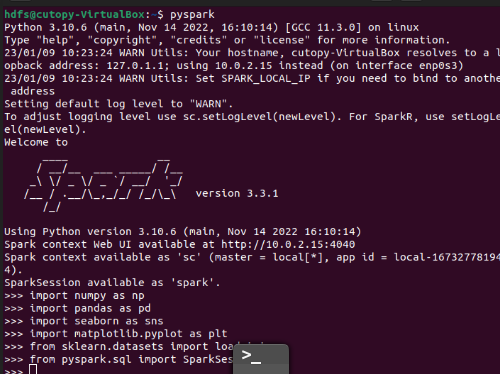
\includegraphics[width=\textwidth]{CutOpyMandalisa/08}
\caption{hasil Tugas individu program machine learning dengan pyspark }
\label{gam:perkuliahan-05-01}
\end{figure}

\begin{figure}[!ht]
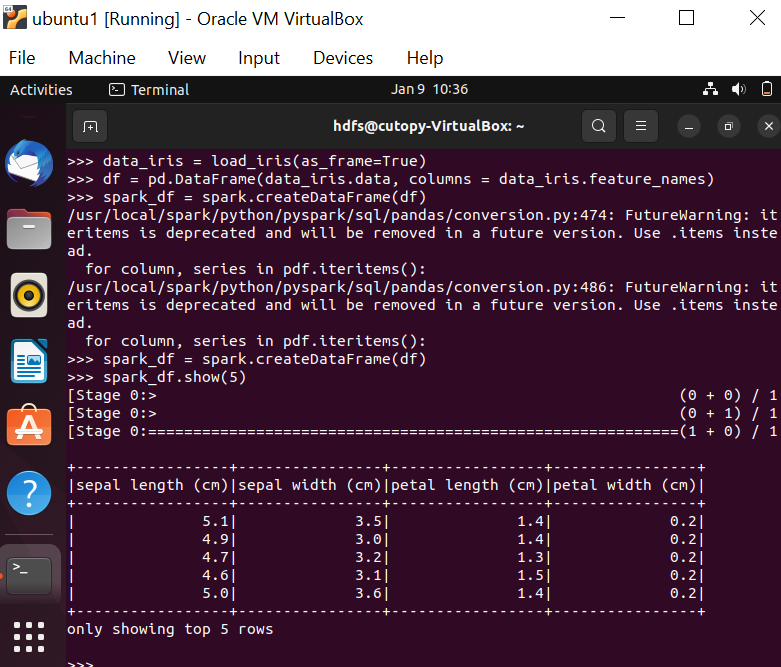
\includegraphics[width=\textwidth]{CutOpyMandalisa/09}
\caption{hasil Tugas individu program machine learning dengan pyspark }
\label{gam:perkuliahan-05-01}
\end{figure}

\item Kesimpulan\\
% berikan kesimpulan dari praktikum yang telah dikerjkan
pada praktikum ini berhasil memunculkan tabel pertama dan tabel yang kedua masih belum berhasil.tabel yang muncul adalah tabel dari load data iris dan tabel penentuan nilai k asemmble data.
\end{enumerate}